\documentclass{../../oss-apphys}
\usepackage[siunitx]{circuitikz}

\begin{document}
\genheader

\gentitle{1 \& C}{CIRCUIT ANALYSIS}{12 \& 13}

\genmultidirections

\gengravity

\raggedcolumns
\begin{multicols}{2}

  \textbf{Questions 1 to 4}  
  \begin{center}
    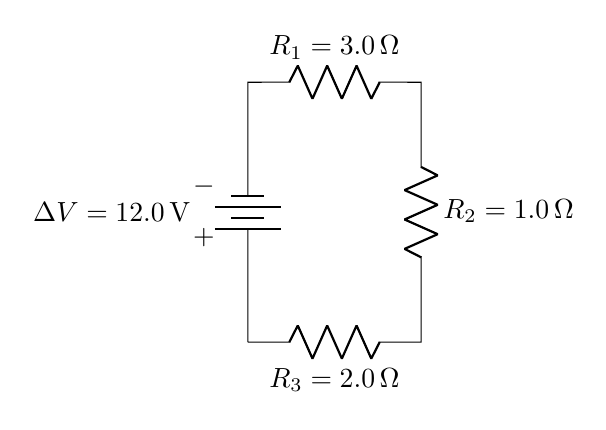
\begin{tikzpicture}[american voltages,scale=1.1]
      \draw(0,0)
      to[battery=\mbox{$\Delta V=\SI{12.0}{\volt}$}] (0,3)
      to[R=\mbox{$R_1=\SI{3.0}{\ohm}$}] (2,3)
      to[R=\mbox{$R_2=\SI{1.0}{\ohm}$}] (2,0)
      to[R=\mbox{$R_3=\SI{2.0}{\ohm}$}] (0,0);
    \end{tikzpicture}
  \end{center}
  
  \begin{enumerate}[leftmargin=18pt]

  \item What is the current flowing through the circuit shown in the diagram?
    \begin{enumerate}[noitemsep,topsep=0pt,leftmargin=18pt,label=(\Alph*)]
    \item\SI{1}{A}
    \item\SI{2}{A}
    \item\SI{4}{A}
    \item\SI{6}{A}
    \item\SI{12}{A}
    \end{enumerate}
    
  \item Which of the following statements is true about the circuit shown in the
    diagram?
    \begin{enumerate}[noitemsep,topsep=0pt,leftmargin=18pt,label=(\Alph*)]  
    \item The voltage drop is greatest across $R_1$, but $R_1$ has the least
      amount of current flowing through it.
    \item The voltage drop is greatest across $R_2$, but $R_2$ has the least
      amount of current flowing through it.
    \item The voltage drop is greatest across $R_3$, but $R_3$ has the least
      amount of current flowing through it.
    \item The voltage drops and current are equal across all resistors.
    \item The voltage drop is greatest across $R_1$, but the current is equal at
      all points in the circuit.
    \end{enumerate}

    \columnbreak
    
  \item In this diagram, what is the power dissipated by all of the resistors in
    the circuit?
    \begin{enumerate}[noitemsep,topsep=0pt,leftmargin=18pt,label=(\Alph*)]  
    \item\SI{2}{W}
    \item\SI{6}{W}
    \item\SI{12}{W}
    \item\SI{24}{W}
    \item\SI{48}{W}
    \end{enumerate}
  
  \item In the diagram, what is the voltage drop across the third resistor
    ($R_3$)?
    \begin{enumerate}[noitemsep,topsep=0pt,leftmargin=18pt,label=(\Alph*)]  
    \item\SI{2}{V}
    \item\SI{3}{V}
    \item\SI{4}{V}
    \item\SI{6}{V}
    \item\SI{12}{V}
    \end{enumerate}

  \item Which of the following statements best summarizes a series circuit
    with three different resistances?
    \begin{enumerate}[noitemsep,topsep=0pt,leftmargin=18pt,label=(\Alph*)]
    \item In all parts of the circuit, the resistances are different, the
      voltage drops are the same, and the current is different.
    \item In all parts of the circuit, the resistances are the same, the voltage
      drops are the same, and the current is different.
    \item In all parts of the circuit, the resistances are different, the
      voltage drops are different, and the current is the same.
    \item In all parts of the circuit, the resistances are different, the
      voltage drops are the same, and the current is the same.
    \item In all parts of the circuit, the resistances are the same, the
      voltage drops are the same, and the current is the same.
    \end{enumerate}
  \end{enumerate}
  \columnbreak

  \textbf{Questions 6-9}
  \begin{center}
    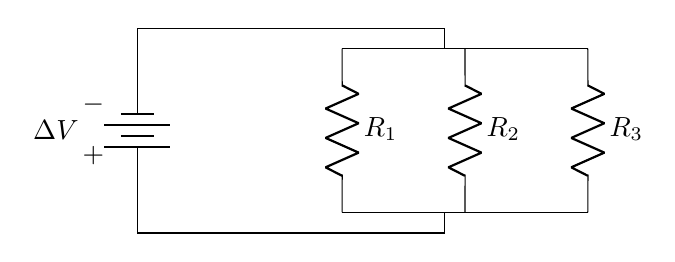
\begin{tikzpicture}[american voltages,scale=1.3]
      \draw(0,0) to[battery=$\Delta V$] (0,2)--(3,2)--(3,1.8);
      \draw(2,1.8)--(4.4,1.8);
      \draw(2,0.2)--(4.4,0.2);
      \draw(2,1.8) to[R=$R_1$] (2,0.2);
      \draw(3.2,1.8) to[R=$R_2$] (3.2,0.2);
      \draw(4.4,1.8) to[R=$R_3$] (4.4,0.2);
      \draw(3,0.2)--(3,0)--(0,0);
    \end{tikzpicture}
    
    \vspace{.1in}$\Delta V=\SI{12.0}{V}$, $R_1=\SI{10.0}{\ohm}$,\\
    $R_2=\SI{6.0}{\ohm}$, $R_3=\SI{8.0}{\ohm}$
  \end{center}

  \begin{enumerate}[leftmargin=18pt]
    \setcounter{enumi}{5}

  \item For the circuit in the diagram, which of the following expressions will
    describe the amount of current flowing through the resistors?
    \begin{enumerate}[noitemsep,topsep=0pt,leftmargin=18pt,label=(\Alph*)]
    \item $I_1=I_2=I_3$
    \item $I_3>I_2>I_1$
    \item $I_1>I_2<I_3$
    \item $I_2>I_1>I_3$
    \item $I_1<I_2<I_3$
    \end{enumerate}
    
  \item For the circuit in the diagram, what is the equivalent resistance?
    \begin{enumerate}[noitemsep,topsep=0pt,leftmargin=18pt,label=(\Alph*)]
      \item\SI{0.040}{\ohm}
      \item\SI{0.40}{\ohm}
      \item\SI{1.0}{\ohm}
      \item\SI{2.6}{\ohm}
      \item\SI{24}{\ohm}
    \end{enumerate}
    
  \item For the circuit in the diagram, what is the total current?
    \begin{enumerate}[noitemsep,topsep=0pt,leftmargin=18pt,label=(\Alph*)]
    \item\SI{0.5}{A}
    \item\SI{4.6}{A}
    \item\SI{12}{A}
    \item\SI{30}{A}
    \item\SI{300}{A}
    \end{enumerate}
    
  \item For the circuit in the diagram, the third resistor ($R_3$) dissipates
    how much energy each second?
    \begin{enumerate}[noitemsep,topsep=0pt,leftmargin=18pt,label=(\Alph*)]
    \item\SI{12}{W}
    \item\SI{14}{W}
    \item\SI{46}{W}
    \item\SI{212}{W}
    \item\SI{300}{W}
    \end{enumerate}

    \columnbreak
    
  \item Two resistors made of the same material are shown in the figure. A
    current of $I$ flows through the left resistor when connected to a
    potential difference of $V$. What current will flow through the right
    resistor when connected to the same potential?

    \vspace{-.2in}
    \begin{center}
      \pic{.45}{resistors.png}
    \end{center}
    \begin{enumerate}[noitemsep,topsep=0pt,leftmargin=18pt,label=(\Alph*)]
    \item $I/2$
    \item $I/4$
    \item $I$
    \item $2I$
    \item $4I$
    \end{enumerate}
  \end{enumerate}

  \textbf{Questions 11 and 12}
  
  \begin{center}
    \pic{.45}{resistors-series.png}
  \end{center}
  
  \begin{enumerate}[leftmargin=18pt]
    \setcounter{enumi}{10}
  \item Which is the correct ranking of the currents for the resistors?
    \begin{enumerate}[noitemsep,topsep=0pt,leftmargin=18pt,label=(\Alph*)]
    \item$I_A = I_B = I_C$
    \item$I_A > I_B > I_C$
    \item$I_C > I_A = I_B$
    \item$I_C > I_B > I_A$
    \item$I_C < I_B < I_A$
    \end{enumerate}

  \item Which is the correct ranking of the potential differences of the
    resistors?
    \begin{enumerate}[noitemsep,topsep=0pt,leftmargin=18pt,label=(\Alph*)]
    \item $V_A = V_B = V_C$
    \item $V_A > V_B > V_C$
    \item $V_A = V_B > V_C$
    \item $V_C > V_B > V_A$
    \item $V_C < V_B < V_A$
    \end{enumerate}
  \end{enumerate}

  \columnbreak
  
  \textbf{Questions 13-14}

  \begin{center}
    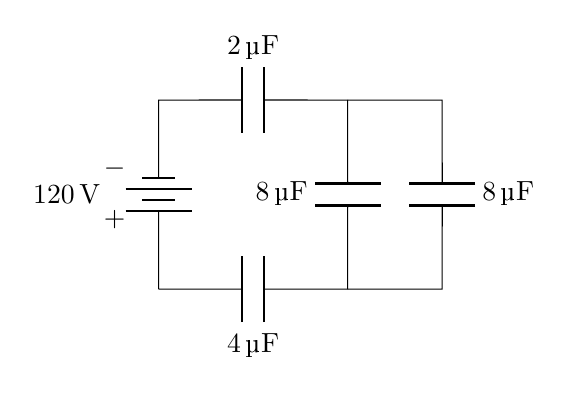
\begin{tikzpicture}[american voltages,scale=1.2]
      \draw(0,0) to[battery=120<\volt>] (0,2) to[C=2<\micro\farad>](2,2)
      to[C,l_=8<\micro\farad>](2,0) to[C=4<\micro\farad>](0,0);
      \draw(2,2)--(3,2) to[C=8<\micro\farad>] (3,0)--(2,0);
    \end{tikzpicture}
  \end{center}

  \begin{enumerate}[leftmargin=18pt]
    \setcounter{enumi}{12}
  \item The equivalent capacitance of this circuit is
    \begin{enumerate}[noitemsep,topsep=0pt,leftmargin=18pt,label=(\Alph*)]
    \item\SI{7/4}{\micro\farad}
    \item\SI{4/7}{\micro\farad}
    \item\SI{21/16}{\micro\farad}
    \item\SI{10}{\micro\farad}
    \item\SI{22}{\micro\farad}
    \end{enumerate}
    
  \item The charge stored on the \SI{2}{\micro\farad} capacitor is most nearly
    \begin{enumerate}[noitemsep,topsep=0pt,leftmargin=18pt,label=(\Alph*)]
    \item\SI{6}{\micro\coulomb}
    \item\SI{12}{\micro\coulomb}
    \item\SI{22}{\micro\coulomb}
    \item\SI{36}{\micro\coulomb}
    \item\SI{120}{\micro\coulomb}
    \end{enumerate}
    
    \columnbreak

  \item A capacitor $C_0$ is connected to a battery and stores charge. If the
    space between the capacitor plates is filled with oil, which of the
    following quantities increase?
    \begin{enumerate}[noitemsep,topsep=0pt,leftmargin=18pt,label=(\Alph*)]
    \item Capacitance and voltage across the plates
    \item Charge and voltage across the plates
    \item Capacitance and electric field between the plates
    \item Capacitance and charge on the plates
    \item Electric field between the plates and voltage across the plates
    \end{enumerate}
  \end{enumerate}

  \textbf{Question 16--17}
  
  The circuit shows a capacitor, a battery, and a resistor. Switch $S$ is first
  connected to point $a$ to charge the capacitor, then a long time later
  switched to point $b$ to discharge the capacitor through the resistor.
  \begin{center}
    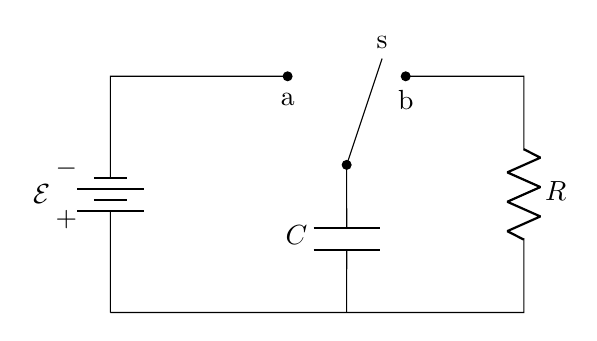
\begin{tikzpicture}[american voltages,scale=1.5]
      \draw(0,0) to[battery=$\mathcal{E}$](0,2) to[short,-*] (1.5,2);
      %node[pos=1,above]{a};
      \draw(2.5,2) to[short,*-] (3.5,2) to[R=$R$,] (3.5,0)--(0,0);
      \draw(2,0) to[C=$C$,-*] (2,1.25);
      \draw(2,1.25)--(2.3,2.15) node[pos=1,above]{s};
      \node at (1.5,1.8) (a){a};
      \node at (2.5,1.8) (b){b};
    \end{tikzpicture}
  \end{center}
  
  \begin{enumerate}[leftmargin=18pt]
    \setcounter{enumi}{15}
  \item The time constant $\tau$ for discharging the capacitor through the
    resistor could be decreased (faster discharge) by
    \begin{enumerate}[noitemsep,topsep=0pt,leftmargin=18pt,label=(\Alph*)]
    \item placing another resistor in series with the first resistor
    \item placing another resistor in parallel with the first resistor
    \item placing another capacitor in parallel with the first capacitor
    \item placing another battery in series in the same direction with the
      first battery
    \item increasing both R and C
    \end{enumerate}

  \item The maximum current through the resistor is
    \begin{enumerate}[noitemsep,topsep=0pt,leftmargin=18pt,label=(\Alph*)]
    \item $\mathcal{E}/2R$
    \item $\mathcal{E}/R$
    \item $\mathcal{E}/RC$
    \item $\mathcal{E}/2RC$
    \item $C\mathcal{E}/R$
    \end{enumerate}
  \end{enumerate}
  \columnbreak
  \textbf{Questions 18--20}
  \begin{enumerate}[leftmargin=18pt]
    \setcounter{enumi}{17}
  \item The spherical capacitor shown consists of a conducting shell of radius a
    inside a larger conducting shell of radius b. A charge $−Q$ is placed on the
    inner sphere and a charge $+Q$ is placed on the outer shell. The
    capacitance of the capacitor is $C_0$. The magnitude of the electric field
    $E$ at a distance $r$ between the spheres is
    \begin{center}
      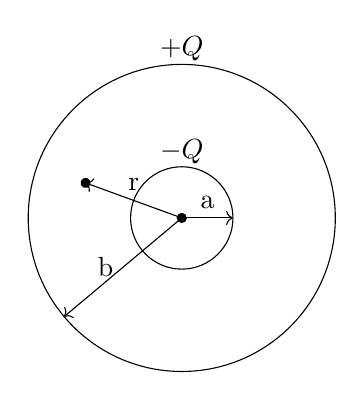
\begin{tikzpicture}[scale=.65]
        \draw(0,0) circle(1);
        \draw(0,0) circle(3);
        \fill(0,0) circle(.1);
        \draw[->](0,0)--(1,0) node[midway,above]{a};
        \draw[->,rotate=-140](0,0)--(3,0) node[midway,left]{b};
        \begin{scope}[rotate=160]
          \draw[->](0,0)--(2,0) node[midway,above]{r};
          \fill(2,0) circle(.1);
        \end{scope}
        \node at (0,3.3) (a){$+Q$};
        \node at (0,1.3) (b){$-Q$};
      \end{tikzpicture}
    \end{center}
    \begin{enumerate}[noitemsep,topsep=0pt,leftmargin=18pt,label=(\Alph*)]    
    \item $\displaystyle\frac{Q}{4\pi\epsilon_0r^2}$
    \item $\displaystyle\frac{Q}{4\pi\epsilon_0r}$
    \item $\displaystyle\frac{Q}{4\pi\epsilon_0a^2}$
    \item $\displaystyle\frac{Q}{4\pi\epsilon_0b^2}$
    \item zero
    \end{enumerate}

  \item The bottom half of the space between the spheres is filled with oil of
    dielectric constant $\kappa=3$, creating two capacitors connected to each
    other. Which of the following is true of the two capacitors?
    \begin{center}
      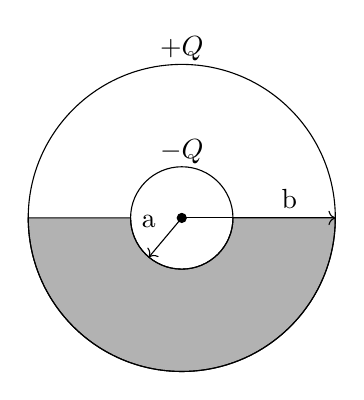
\begin{tikzpicture}[scale=.65]
        \draw[fill=gray!60](-1,0)--(-3,0) arc(180:360:3)--(1,0) arc(0:-180:1);
        \draw(0,0) circle(1);
        \draw(0,0) circle(3);
        \fill(0,0) circle(.1);
        \draw[->,rotate=230](0,0)--(1,0) node[midway,above left]{a};
        \draw[->](0,0)--(3,0) node[pos=0.7,above]{b};
        \node at (0,3.3) (a){$+Q$};
        \node at (0,1.3) (b){$-Q$};
      \end{tikzpicture}
    \end{center}
    \begin{enumerate}[noitemsep,topsep=0pt,leftmargin=18pt,label=(\Alph*)]
    \item They are connected in series.
    \item They are connected in parallel.
    \item The total capacitance has not changed.
    \item The total capacitance of the spheres has decreased.
    \item The total capacitance is now zero.
    \end{enumerate}
    \columnbreak
    
  \item With the bottom half of the space between the spheres having been
    filled with oil of dielectric constant $\kappa=3$, the new capacitance of
    the spheres is
    \begin{enumerate}[noitemsep,topsep=0pt,leftmargin=18pt,label=(\Alph*)]
    \item zero
    \item $C_0$
    \item $2C_0$
    \item $3C_0$
    \item $4C_0$
    \end{enumerate}
    
%    \columnbreak
    
  \item A battery of voltage $V_0$ is attached to two parallel conducting
    plates. Charge is distributed on the plates, and then the battery is
    removed. A dielectric is then inserted between the plates, filling the
    space. Which of the following decreases after the battery is removed and the
    dielectric is inserted to fill the space between the plates?
    \begin{enumerate}[noitemsep,topsep=0pt,leftmargin=18pt,label=(\Alph*)]
    \item Capacitance
    \item Charge on the plates
    \item Net electric field between the plates
    \item Area of the plates
    \item Separation distance between the plates
    \end{enumerate}

  \item Circuit I and Circuit II shown each consist of a capacitor and a
    resistor. A battery is connected across a and b, and then removed. Which of
    the following statements is true of the circuits?
    \begin{center}
      Circuit I\\
      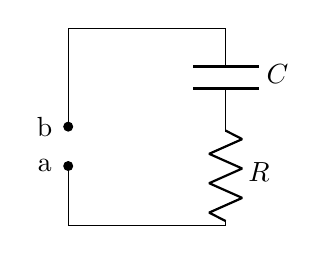
\begin{tikzpicture}
        \draw(0,1.25) to[short,*-](0,2.5)--(2,2.5) to[C=$C$](2,1.25)
        to[R=$R$](2,0)--(0,0) to[short,-*](0,0.75);
        \node at (-0.3,0.75) {a};
        \node at (-0.3,1.25) {b};
      \end{tikzpicture}
      
      Circuit II\\
      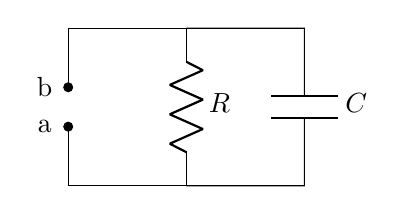
\begin{tikzpicture}
        \draw(0,1.25) to[short,*-](0,2)--(1.5,2) to[R=$R$](1.5,0)--(0,0)
        to[short,-*](0,0.75);
        \draw(1.5,2)--(3,2) to[C=$C$](3,0)--(1.5,0);
        \node at (-0.3,0.75) {a};
        \node at (-0.3,1.25) {b};
      \end{tikzpicture}
    \end{center}
    \begin{enumerate}[noitemsep,topsep=0pt,leftmargin=18pt,label=(\Alph*)]
    \item Circuit I and Circuit II will both retain stored energy when the
      battery is removed.
    \item Neither Circuit I nor Circuit II will retain stored energy when the
      battery is removed.
    \item Only Circuit I will retain stored energy when the battery is
      removed.
    \item Only Circuit II will retain stored energy when the battery is
      removed.
    \item Current will continue to flow in both circuits after the battery is
      removed.
    \end{enumerate}
    
  \end{enumerate}
\end{multicols}

\newpage
\begin{center}
  {\Large
    \textbf{AP\textsuperscript{\textregistered} Physics C: Circuit Analysis\\
      Student Answer Sheet for Multiple-Choice Section}
  }
  
  %begin{minipage}{.2\textwidth}
  \vspace{.2in}
  \bgroup
  \begin{tabular}{>{\centering}m{1.3cm} >{\centering}m{1.7cm}}
    No. & Answer
  \end{tabular}\\
  \def\arraystretch{1.5}
  \begin{tabular}{|>{\centering}m{1.3cm}|>{\centering}m{1.7cm}|}
    \hline
    1 & \\ \hline
    2 & \\ \hline
    3 & \\ \hline
    4 & \\ \hline
    5 & \\ \hline
    6 & \\ \hline
    7 & \\ \hline
    8 & \\ \hline
    9 & \\ \hline
    10 & \\ \hline
    11 & \\ \hline
    12 & \\ \hline
    13 & \\ \hline
    14 & \\ \hline
    15 & \\ \hline
    16 & \\ \hline
    17 & \\ \hline
    18 & \\ \hline
    19 & \\ \hline
    20 & \\ \hline
    21 & \\ \hline
    22 & \\ \hline
  \end{tabular}
  \egroup
  %end{minipage}
\end{center}
\newpage

\newpage

\genfreetitle{1 \& C}{CIRCUIT ANALYSIS}{4}

\genfreedirections{10}

\begin{enumerate}[leftmargin=15pt]

\item The circuit in the figure consists of three capacitors
  (\SI{3}{\micro\farad}, \SI{4}{\micro\farad}, and \SI{6}{\micro\farad})
  connected to a \SI{200}{\volt} battery.
  
  \begin{minipage}{0.3\textwidth}
    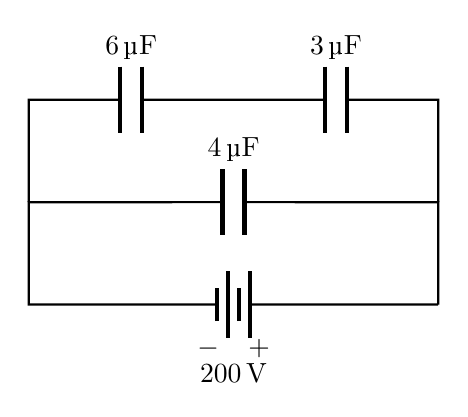
\begin{tikzpicture}[american voltages,scale=1.3]
      \draw[thick](4,0) to[battery=200<\volt>](0,0)--(0,1)
      to[C=4<\micro\farad>](4,1)--(4,0);
      \draw[thick](0,1)--(0,2) to[C=6<\micro\farad>] (2,2)
      to[C=3<\micro\farad>] (4,2)--(4,1);
    \end{tikzpicture}
  \end{minipage}
  \begin{minipage}{.68\textwidth}
    \begin{enumerate}[noitemsep]
    \item Calculate the equivalent capacitance of the combined three
      capacitors.
    \item Calculate the total energy stored in the \SI{6}{\micro\farad} and
      \SI{3}{\micro\farad} capacitor combination.
    \end{enumerate}
  \end{minipage}
  \vspace{1.5in}
  
\item A \SI{60}{\micro\farad} capacitor is charged to \SI{12}{\volt}. The
  capacitor is then removed from the battery and the plate separation is
  increased from \SI{2.0}{mm} to \SI{3.5}{mm}.
  \begin{enumerate}[noitemsep]
  \item What is the charge on the capacitor?
  \item How much energy was originally stored in the capacitor?
  \item By how much is the energy increased when the plate separation is
    changed?
  \end{enumerate}
  \newpage

\item Find the current in each part of the circuit shown in the figure below.
  \begin{center}
    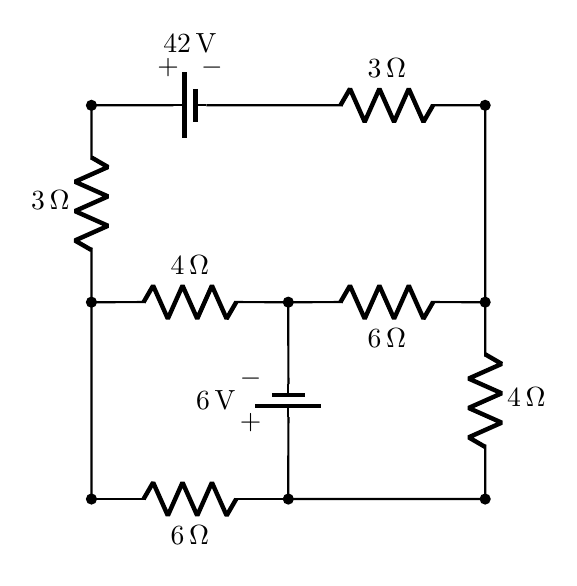
\begin{tikzpicture}[american voltages,scale=1.25]
      \draw[thick](0,0) to[short,*-](0,2) to[R=3<\ohm>,*-] (0,4)
      to[battery1=42<\volt>,*-](2,4) to[R=3<\ohm>] (4,4) to[short,*-](4,2)
      to[R=4<\ohm>,*-](4,0) to[short,*-](2,0) to[battery1=6<\volt>,*-](2,2)
      to[R,l_=4<\ohm>,*-](0,2);
      \draw[thick](0,0) to[R,l_=6<\ohm>](2,0);
      \draw[thick](2,2) to[R,l_=6<\ohm>](4,2);
    \end{tikzpicture}
  \end{center}
  \newpage
  
%\item The capacitor in the circuit is initially uncharged. Find the current
%  through the battery
%  \begin{enumerate}[noitemsep]
%  \item Immediately after the switch is closed
%  \item A long time after the switch is closed 
%  \end{enumerate}
%
%  \begin{center}
%    \begin{tikzpicture}[scale=1.25,american voltages]
%      \draw[thick] (0,0) to[battery1=12<\volt>,*-*] (0,2) to[R=4<\ohm>] (2,2)
%      to[short,*-](2.46,2.3);
%      \draw[thick](2.5,2) to[short,*-*] (3,2) to[short,-*] (4,2)
%      to[C=6<\micro\farad>,-*] (4,0)--(0,0);
%      \draw[thick] (3,0) to[R=8<\ohm>,*-] (3,2);
%    \end{tikzpicture}
%  \end{center}


\item The figure shows a circuit with two resistors, a battery, a capacitor,
  and a switch. Originally, the switch is open, and the capacitor is
  uncharged.

  \vspace{-.5cm}
  \begin{center}
    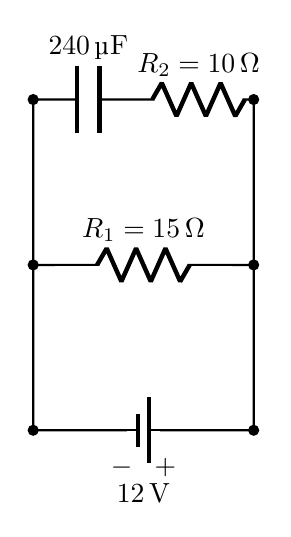
\begin{tikzpicture}[scale=1.4,american voltages]
      \draw[thick] (2,0) to[battery1=12<\volt>,*-*] (0,0)
      to[short,-*] (0,1.5) to[R=\mbox{$R_1=\SI{15}{\ohm}$},-*] (2,1.5)--(2,0);
      \draw[thick](0,1.5) to[short,-*] (0,3) to[C=240<\micro\farad>] (1,3)
      to[R=\mbox{$R_2=\SI{10}{\ohm}$},-*] (2,3)--(2,1.5);
    \end{tikzpicture}
  \end{center}
  
  \begin{enumerate}[noitemsep]
  \item Complete the voltage-current-resistance-power (VIRP) chart for
    the circuit immediately after the switch is closed.
    \bgroup
    \def\arraystretch{2}
    
    {\large
      \begin{center}
        \begin{tabular}{l|m{1.2cm}|m{1.2cm}|m{1.2cm}|m{1.2cm}}
          \hline
          \textbf{Location} & \textbf{\emph{V}} & \textbf{\emph{I}} &
          \textbf{\emph{R}} & \textbf{\emph{P}}\\ \hline
          1 & & & \SI{15}{\ohm} & \\ \hline
          2 & & & \SI{10}{\ohm} & \\ \hline
          Total for Circuit & \SI{12}{\volt}& & & \\\hline
        \end{tabular}
      \end{center}
    }
    \egroup
  \item Complete the voltage-current-resistance-power (VIRP) chart for
    the circuit after the switch is closed for a long time.
        \bgroup
    \def\arraystretch{2}
    
    {\large
      \begin{center}
        \begin{tabular}{l|m{1.2cm}|m{1.2cm}|m{1.2cm}|m{1.2cm}}
          \hline
          \textbf{Location} & \textbf{\emph{V}} & \textbf{\emph{I}} &
          \textbf{\emph{R}} & \textbf{\emph{P}}\\ \hline
          1 & & & \SI{15}{\ohm} & \\ \hline
          2 & & & \SI{10}{\ohm} & \\ \hline
          Total for Circuit & \SI{12}{\volt}& & & \\\hline
        \end{tabular}
      \end{center}
    }
    \egroup
  \item What is the energy stored in the capacitor after the switch has
    been closed a long time?
  \end{enumerate}
\end{enumerate}


\end{document}
